\section{Simplicial Abelian Groups}
\label{sec:Simplicial Abelian Groups}

Before defining \emph{simplicial abelian groups}, we will first discuss the more general notion of \emph{simplicial sets}. There are generally two definitions of simplicial sets, an abstract one and a very explicit one. We will start with the abstract one, luckily it can still be visualised in pictures, then we will derive the explicit definition.

\subsection{Abstract definition}
\begin{definition}
	We define a category $\DELTA$, where the objects are the finite ordinals $[n] = \{0, \dots, n\}$ for $n \in \N$ and maps are monotone increasing functions: $\Hom{\DELTA}{[n]}{[p]} = \{ f : [n] \to [p] \I f(i) \leq f(j) \text{ for all } i < j \}$.
\end{definition}

There are two special kinds of maps in $\DELTA$, the so called \emph{face} and \emph{degeneracy} maps, defined as (resp.):

\begin{align*}
	\delta_i: [n] \to [n+1], k & \mapsto \begin{cases} k & \text{if } k < i;\\ k+1 & \text{if } k \geq i. \end{cases} \hspace{0.5cm} 0 \leq i \leq n+1, \text{ and} \\
	\sigma_i: [n+1] \to [n], k & \mapsto \begin{cases} k & \text{if } k \leq i;\\ k-1 & \text{if } k > i. \end{cases} \hspace{0.5cm} 0 \leq i \leq n
\end{align*}

for each $n \in \N$. The nice things about these maps is that every map in $\DELTA$ can be decomposed to a composition of these maps. \todo{sAb: Epi-mono factorization of $\DELTA$} So in a sense, these are all the maps we need to consider. We can now picture the category $\DELTA$ as in figure~\ref{fig:delta_cat}.

\begin{figure}[h!]
	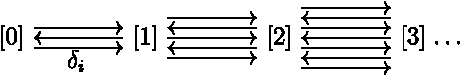
\includegraphics{delta_cat}
	\caption{The category $\DELTA$ with the face and degeneracy maps.}
	\label{fig:delta_cat}
\end{figure}

Althoug this is a very abstract definition, a more geometric intuition can be given. In $\DELTA$ we can regard $[n]$ as an abstract version of the $n$-simplex $\Delta^n$. The face maps $\delta_i$ are then exactly maps which point out how we can embed $\Delta^n$ in $\Delta^{n+1}$. This is shown in figure~\ref{fig:delta_cat_geom}. This picutre shows the images of the face maps, for example the image of $\delta_3$ from $[2]$ to $[3]$ is the set $\{0,1,2\}$, which is the bottom face of the tetrahedron. The degeneracy maps are harder to visualize, one can think of them as collapsing maps, where two points are identified with eachother. \todo{sAb: how to draw $\sigma_i$?}

\begin{figure}
	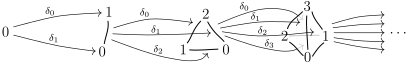
\includegraphics{delta_cat_geom}
	\caption{The category $\DELTA$ with the face maps shown in a geometric way.}
	\label{fig:delta_cat_geom}
\end{figure}

This category $\DELTA$ will act as a protoype for these kind of geometric structures in other categories. This leads to the following definition.

\begin{definition}
	An \emph{simplicial set} $X$ is a contravariant functor:
	$$X: \DELTA \to \Set.$$
	(Or equivalently a covariant functor $X: \DELTA^{op} \to \Set.$)
\end{definition}

So the category of all simplicial sets, $\sSet$, is the functor category $\Set^{\DELTA^{op}}$, where morphisms are natural transformations. Because the face and degeneracy maps give all the maps in $\DELTA$ it is sufficient to define images of $\delta_i$ and $\sigma_i$ in order to define a functor $X: \DELTA^{op} \to \Set$. And hence we can picture a simplicial set as done in figure~\ref{fig:simplicial_set}. Comparing this to figure~\ref{fig:delta_cat} we see that the arrows are reversed, because $X$ is a contravariant functor.

\begin{figure}
	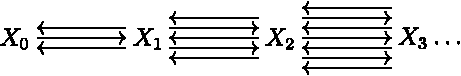
\includegraphics{simplicial_set}
	\caption{A simplicial set.}
	\label{fig:simplicial_set}
\end{figure}


\subsection{Explicit definition}
Of course the maps $\delta_i$ and $\sigma_i$ in $\DELTA$ satisfy certain equations, these are the so called \emph{simplicial equations}.
\todo{sAb: Is \emph{simplicial equations} really a thing?}

\begin{lemma}
	The face and degeneracy maps in $\DELTA$ satisfy the simplicial equations, ie.:
	\begin{align}
		\delta_j\delta_i &= \delta_i\delta_{j-1}  \hspace{0.5cm} \text{ if } i < j,\\
		\sigma_j\delta_i &= \delta_i\sigma_{j-1}  \hspace{0.5cm} \text{ if } i < j,\\
		\sigma_j\delta_j &= \sigma_j\delta_{j+1} = \id,\\
		\sigma_j\delta_i &= \delta_{i-1}\sigma_j  \hspace{0.5cm} \text{ if } i > j+1,\\
		\sigma_j\sigma_i &= \sigma_i\sigma_{j+1}  \hspace{0.5cm} \text{ if } i \leq j.
	\end{align}
\end{lemma}
\begin{proof}
	By writing out the definitions given above. \todo{sAb: this is a bit rude, maybe write out some of it...}
\end{proof}

Because a simplicial set $X$ is a contravariant functor, these equations (which only consist of compositions and identities) also hold in its image. For example the first equation would look like: $ X(\delta_i)X(\delta_j) = X(\delta_{j-1})X(\delta_i) $ for $ i < j$. This can be used for an explicit definition of simplicial sets. In this definition a simplicial set $X$ consists of a collection sets $X_n$ together with the face and degeneracy maps. More precisely:

\begin{definition}
	\emph{(Explicitly)} An simplicial set $X$ consists of a collection sets $A_n$ together with functions $d_i : X_n \to X_{n-1}$ and $s_i : X_n \to X_{n+1}$ for $0 \leq i \leq n$ and $n \in \N$, such that:
	\begin{align}
		d_i d_j &= d_{j-1} d_i  \hspace{0.5cm} \text{ if } i < j,\\
		d_i s_j &= s_{j-1} d_i  \hspace{0.5cm} \text{ if } i < j,\\
		d_j s_j &= d_{j+1} s_j = \id,\\
		d_i s_j &= s_j d_{i-1}  \hspace{0.5cm} \text{ if } i > j+1,\\
		s_i s_j &= s_{j+1} s_i  \hspace{0.5cm} \text{ if } i \leq j.
	\end{align}
\end{definition}

It is already indicated that a functor from $\DELTA^{op}$ to $\Set$ is determined when the images for the face and degeneracy maps in $\DELTA$ are provided. So this gives a way of restoring the first definition from this one. Conversely, we can apply functorialty to obtain the second definition from the first. So these definitions are the same \todo{sAb: is it ok not to prove this?}. From now on we will denote $X([n])$ by $X_n$, $X(\sigma_i)$ by $s_i$ and $X(\delta_i)$ by $d_i$, whenever we have a simplicial set $X$. For any other map $\beta : [n] \to [p]$ we will denote the induced map by $\beta^\ast : X_p \to X_n$.

When using a simplicial set to construct another object, it is often handy to use this second definition, as it gives you a very concrete objects to work with. On the other hand, constructing this might be hard (as you would need to provide a lot of details), in this case we will often use the more abstract definition.

\todo{sAb: Note that $s_i$ is a monomorphism because of (3)}

\subsection{The standard $n$-simplex}
There are very important simplicial sets:

\begin{definition}
	The standard $n$-simplex is given by:
	$$\Delta[n] = \Hom{\DELTA}{-}{[n]} : \DELTA^{op} \to \Set.$$
\end{definition}

Note that indeed $\Hom{\DELTA}{X}{[n]} \in \Set$, because the collection of morphisms in a category is per definition a set. We do not need to specify the face or degeneracy maps, as we already know that $\mathbf{Hom}$ is a functor (in both arguments). Still it is useful to write out some cases.

\begin{example}
	We will compute how $\Delta[0]$ look like. Note that $[0]$ is an one-element set, so for any set $X$, there is only one function $\ast : X \to [0]$. Hence $\Delta[0]_n = \{\ast\}$ for all $n$. The face and degeneracy maps are now functions from $\{\ast\}$ to $\{\ast\}$. Again there is only one, namely $\id : \{\ast\} \to \{\ast\}$. This gives:
	$$ \Delta[0] = \{\ast\} \to \{\ast\} \to \{\ast\} \to \cdots. $$
\end{example}

\begin{example}
	$\Delta[1]$ is a bit more interesting, but still not too hard. We will compute the first three abelian groups $\Delta[1]_0$, $\Delta[1]_1$ and $\Delta[1]_2$. We can use the fact that any monotone increasing map $f: [n] \to [m]$ is a composition of first applying degeneracy maps, and then face maps, ie.: $f: [n] \tot{\sigma_{i_0} \cdots \sigma_{i_M}} [k] \tot{\delta_{j_0} \cdots \delta_{j_N}} [m]$, where $k \leq m, n$.

	For $\Delta[1]_0$ we have to consider maps from $[0]$ to $[1]$, we cannot first apply degeneracy maps (there is no object $[-1]$). So this leaves us with the face maps: $\Delta[1]_0 = \{\delta_0, \delta_1\}$. For $\Delta[1]_1$ we of course have the identity function and two functions $\delta_0\sigma_0, \delta_1\sigma_0$. Now $\Delta[1]_2$ are the maps from $[2]$ to $[1]$.

	We will compute the two face maps $d_0$ and $d_1$ from $\Delta[1]_1$ to $\Delta[1]_0$. Recall that the $\mathbf{Hom}$-functor in the first argument (the contravariant argument) works with precomposition. So this gives:
	\begin{align*}
		d_0(id) &= \id \delta_0 = \delta_0 \\
		d_0(\delta_0\sigma_0) &= \delta_0 \sigma_0 \delta_0 = \delta_0 \\
		d_0(\delta_1\sigma_0) &= \delta_0 \sigma_0 \delta_0 = \delta_1.
	\end{align*}
	Where we in the first calculation used the identity law. In the second and third line we used the third simplicial equation, asserting that $\sigma_0 \delta_0 = \id$. Similarly we can calculate the face map $d_1$:
	\begin{align*}
		d_1(id) &= \id \delta_1 = \delta_1 \\
		d_1(\delta_0\sigma_0) &= \delta_0 \sigma_0 \delta_1 = \delta_0 \\
		d_1(\delta_1\sigma_0) &= \delta_0 \sigma_0 \delta_1 = \delta_1.
	\end{align*}

	$$ \Delta[1] =
	\begin{tikzpicture}[baseline=-0.5ex]
	\matrix (m) [matrix of math nodes] { 
		\{\delta_0, \delta_1\} & \{\sigma_0 \delta_0, \id, \sigma_0 \delta_1\} & \{ \} & \cdots \\
	}; 

	\foreach \r in {-5, 5} \draw [raise line=\r, <-] (m-1-1) -> (m-1-2);
	\foreach \r in {0} \draw [raise line=\r, ->] (m-1-1) -> (m-1-2);

	\foreach \r in {-10, 0, 10} \draw [raise line=\r, <-] (m-1-2) -> (m-1-3);
	\foreach \r in {-5, 5} \draw [raise line=\r, ->] (m-1-2) -> (m-1-3);

	\foreach \r in {-15, -5, 5, 15} \draw [raise line=\r, <-] (m-1-3) -> (m-1-4);
	\foreach \r in {-10, 0, 10} \draw [raise line=\r, ->] (m-1-3) -> (m-1-4);
	\end{tikzpicture}.$$
\end{example}

\subsection{Other simplicial objects}
Of course the abstract definition of simplicial abelian group can easily be generalized to other categories. For any category $\cat{C}$ we can consider the functor category $\cat{sC} = \cat{C}^{\DELTA^{op}}$. In this thesis we are interested in the category $\sAb = \Ab^{\DELTA^{op}}$ of simplicial abelian groups. So a simplicial abelian group $A$ is a collection of abelian groups $A_n$, together with face and degeneracy maps, which in this case means group homomorphisms $d_i$ and $s_i$ such that the simplicial equations hold.

As we are interested in simplicial abelian group, it would be nice to make these standard $n$-simplices into simplicial abelian groups. We have seen how to make an abelian group out of any set using the free abelian group. We can use this functor $\Z[-] : \Set \to \Ab$ to induce a functor $\Z^\ast[-] : \sSet \to \sAb$ as shown in the following diagram.
\begin{figure}[h!]
	\begin{tikzpicture}
		\matrix (m) [matrix of math nodes]{
			\DELTA^{op} & \Set \\
			            & \Ab  \\
		};
		\path[->]
		(m-1-1) edge node[auto] {$ X $} (m-1-2)
		(m-1-2) edge node[auto] {$ \Z[-] $} (m-2-2)
		(m-1-1) edge node[auto] {$ X' $} (m-2-2);
	\end{tikzpicture}
	\caption{The simplicial set $X$ can be made into a simplicial abelian group $X'$ by postcomposing with $\Z[-]$}
	\label{fig:diagram_Z}
\end{figure}

\begin{example}
	We can apply this to the standard $n$-simplex $\Delta[1]$. This gives $\Delta[1]_0 \iso \Z^2$, since $\Delta[1]_0$ had two elements, and $\Delta[1]_1 \iso \Z^3$, where the isomorphisms are taken such that:
	\begin{align*}
		\delta_0         &\mapstot{\iso} (1, 0) \\
		\delta_1         &\mapstot{\iso} (0, 1) \\
		\sigma_0\delta_0 &\mapstot{\iso} (1, 0, 0) \\
		\id              &\mapstot{\iso} (0, 1, 0) \\
		\sigma_0\delta_1 &\mapstot{\iso} (0, 0, 1)
	\end{align*}
	The face maps from $\Delta[1]_1$ to $\Delta[1]_0$ under these isomorphisms are then given by:
	\begin{align*}
		d_0(x, y, z) &= (x+y, z) \\
		d_1(x, y, z) &= (x, y+z)
	\end{align*}
\end{example}
